\documentclass[11pt]{article}


\usepackage{fullpage}
\usepackage{amsmath}
\usepackage{amssymb}
\usepackage{color}
\usepackage{tikz}
\usetikzlibrary{decorations.markings}

\date{}

\newcommand{\ans}[1]{\smallskip\color{blue}#1\color{black}\smallskip}

\newcommand{\mys}[2]{\displaystyle\sum_{#1}^{#2}}


\begin{document}

\begin{center}
  \textbf{COMS 311: Homework 3}\\
  \textbf{Due: Oct 12, 11:59pm}\\
  \textbf{Total Points: 100}
  \end{center}

\paragraph{Submission format.\ }
Your submission should be in pdf format.  Name your submission file:
\texttt{<Your-net-id>-311-hw3.pdf}. For instance, if your netid is
\texttt{asterix}, then your submission file will be named
\texttt{asterix-311-hw3.pdf}.

\hrule
\paragraph{Rules for Algorithm Design Problems.\ }
\begin{enumerate}
\item Unless otherwise mentioned, for all algorithm design problems,
  part of the grade depends on runtime. Better runtime will lead to
  higher grade.
\item Unless otherwise mentioned, for all algorithm design problems,
  you are required to write some justification of why your algorithm
  correctly addresses the given problem.
\item You will write pseudo-code for your algorithm. It should not be
  some code in a specific programming language (e.g., Java, C/C++,
  Python).
\item You can use any operation already covered in class-lectures in
  your solution without explicitly writing the algorithm. However, you
  need to use them appropriately (i.e., indicate the inputs to and
  outputs from these algorithms). For instance, you can use
  \texttt{heapifyUp} with input as the index of a heap element and you
  do not need to write the code for \texttt{heapifyUp}. 
\end{enumerate}

\hrule

\medskip

Problems 1--4 are 25pts each. Extra Credit Problem is 20pt. 


\newpage


\begin{enumerate}

  
\item 
In the indomitable gaulish village, druid Getafix had to make several
trips to all village houses everyday. There are walkways between
houses in this village such that Getafix can take several walkways to
any house and also from any house Getafix can take several walkways to
come back to his house.  All walkways in this village are
\emph{directed}, i.e., one may not be able to take the same
walkway to go back and forth between two houses. Everyday Getafix
has to do the following:
\begin{verbatim}
for every house h
   Getafix walks from his house to h
   Getafix delivers magic potion to the house members
   Getafix walks from h to his own house
\end{verbatim}
Write an algorithm to determine the shortest distance Getafix walks
everyday.  You can assume that every walkway is of length $L$.  The input
to your algorithm is the village map with houses and walkways between
them. Here is an example scenario:
\begin{center}
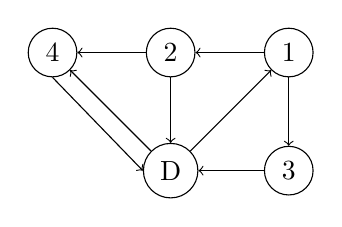
\begin{tikzpicture}[scale=0.5,every node/.style={draw=black,circle}]
\node (D) at (0, 0) {D};
\node (1) at (3, 3) {1};
\node (2) at (0, 3) {2};
\node (3) at (3, 0) {3};
\node (4) at (-3, 3) {4};
\draw [->] (D) to (1);
\draw [->] (1) to (2);
\draw [->] (1) to (3);
\draw [->] (3) to (D);
\draw [->] (D) to (4);
\draw [->] (2) to (4);
\draw [->] (4.south) to (D.west);
\draw [->] (2) to (D);
\end{tikzpicture}
\end{center}

\begin{verbatim}
DFS(v, prevD)
dist(v) = min(prevD + L,dist(v))
  if (!visited(v))
    for all n in v.neighbors
      DFS(n, dist(v))

Getafix(V, E, D)
  total = 0
  for all v in V
  visited(v) = 0
    dist(v) = infinity
  DFS(D, 0) // phase 1: distance to
  for all v in V
    total += dist(v)

  Reverse(E)
  for all v in V
    visited(v) = 0
    dist(v) = infinity
  DFS(D, 0) // phase 2: distance back
  for all v in V
    total += dist(v)

  return total

\end{verbatim}

First, Getaphix finds the shortest path to all houses using DFS and a distance property.
Next we reverse the edges in the graph.
Now, DFS actually finds the shortest path back from all other nodes because the graph is reversed.
Summing all these distances should give the shortest path for Getafix. \\
2 DFSs take O(V + E), 2 resets take O(V), and 1 reversal takes O(E).
Summing these puts Getaphix in O(V + E).

\newpage

\item 
Given a directed graph $G = (V, E)$, a vertex is $k ( < |V|)$ strong
if $k$ vertices can reach the vertex (excluding itself). Write an
algorithm to verify the existence of a $|V|-1$ strong vertex in a
given graph. The input to your algorithm is a directed graph.

\begin{verbatim}
HasStrong(V, E)
  SCCs = Tarjan(V, E)
  V' = all individual components in SCCs
  E' = unique edges connecting components in SCCs

  leaf = null
  for all c in V'
    if |(c, u)| == 0 and leaf != null
      return false
    leaf = c
  
  return true
\end{verbatim}

First we find the SCCs of the input.
Condensed graphs consisting of SCCs are DAGs, so there will at least be one node with 0 neighbors, aka a leaf.
If there are multiple leafs, then these leafs cannot reach other, which gurantees that none of the nodes in the leaf is strong.
If there is a single leaf, then all other nodes in the previous components can reach it, and that leaf is an scc, so all nodes in that leaf is reachable by all other nodes aka strong. \\
Tarjan runs in O(V + E), and checking the neighbors of each SCC is O(V). This puts HasStrong in O(V + E)

\newpage

\item 
Given a connected undirected graph, write an algorithm for verifying
the existence of simple cycle in the graph. A simple cycle is defined
as a sequence of vertices $v_1, \ldots, v_{k}$, where all
vertices are distinct and $\forall i\in [1, k-1], (v_i, v_{i+1}) \in
E$ and $(v_{k}, v_1) \in E$. The input to your algorithm is a connected
undirected graph.

\begin{verbatim}
DFS(v, prev)
  visited(v) = 1
  cycle = 0
  for all n in neighbors(v)
    if n != prev and visited(v)
      return true
    if DFS(n, v) // separate if statements for earlier termination
      return true
  return false

HasSimpleCycle(V, E)
  for each v in V
    visited(v) = 0
  for each v in V
    if !visited(v)
      if DFS(v, null)
        return true
  return false

\end{verbatim}

This is simply a DFS for undirected graph that terminates if it finds a vertex that's already been reached.
This would indicate a cycle, returning true.
If no DFS calls return true, then there is no cycle. \\
This gives HasSimpleCycle O(V + E)


\newpage

\item 
Given a directed graph $G=(V, E)$, we say that it is at least one-way
connected if for every $u_1, u_2\in V$, there exists a path from $u_1$
to $u_2$ or a path from $u_2$ to $u_1$. Write an algorithm to determine
whether $G$ is at least one-way connected. The input to your algorithm
is a directed graph.

Here are couple of scenarios. Graph I is at least one-way connected
and Graph II is not at least one-way connected (in Graph II for pair
of vertices $a$ and $e$, there is no path from $a$ to $e$ and from $e$ to
$a$).
\begin{center}
  \begin{tabular}{c@{\extracolsep{4em}}c}
    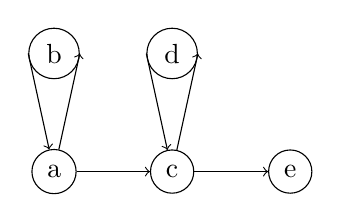
\begin{tikzpicture}[scale=0.5,every node/.style={draw=black,circle}]
\node (a) at (0, 0) {a};
\node (b) at (0, 3) {b};
\node (c) at (3, 0) {c};
\node (d) at (3, 3) {d};
\node (e) at (6, 0) {e};
\draw [->] (a) to (b.east);
\draw [->] (b.west) to (a);
\draw [->] (a) to (c);
\draw [->] (c) to (d.east);
\draw [->] (d.west) to (c);
\draw [->] (c) to (e);
    \end{tikzpicture}
    &
      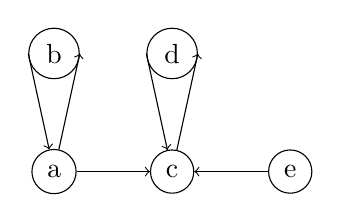
\begin{tikzpicture}[scale=0.5,every node/.style={draw=black,circle}]
\node (a) at (0, 0) {a};
\node (b) at (0, 3) {b};
\node (c) at (3, 0) {c};
\node (d) at (3, 3) {d};
\node (e) at (6, 0) {e};
\draw [->] (a) to (b.east);
\draw [->] (b.west) to (a);
\draw [->] (a) to (c);
\draw [->] (c) to (d.east);
\draw [->] (d.west) to (c);
\draw [->] (e) to (c);
      \end{tikzpicture}
      \\
      (I) & (II) 
    \end{tabular}
  \end{center}

\begin{verbatim}
AtLeastOneWayConnected(V, E)
  SCCs = Tarjan(V, E)
  V' = all individual components in SCCs
  E' = edges connecting components in SCCs

  // compute in degrees
  for each c in V'
    in(c) = 0
  for each e (u, c) in E'
    c.in++

  while (|V'| > 0)
    root = null
    for each c in V'
      if in(c) == 0 && root != null
        root = c
      else
        return false
    for all e (u, root) in E'
      in(u)--
    remove root from V'
  return true
\end{verbatim}

First, we get all the strongly connected components of our graph.
This gives us a condensed graph that is guranteed to be a DAG.
Now we can determine root nodes in our DAG by finding which components have an in degree of 0.
We then remove that root node, update the in degree of all nodes it goes to, and repeat.
If there's ever more than one root node, then we have branches with components where at least one of the branches cannot reach the other.
If there's branches that can reach eachother, then we'd have a cycle, and that's not possible because SCC graphs are DAGs.
So, upon detection of multiple root nodes, we return false, else if we are able to clear all nodes, we can return true. \\
Tarjan takes O(V + E), then we perform initializations in O(V), then calculating in degrees in O(E).
In the worst case for finding each root node, we must make $|V| - k$ comparisons, where k is the nubmer of nodes removed.
So, it could take $|V| + (|V| - 1) + (|V| - 2) + ... + 1$ comparisons to remove all root nodes giving $|V|(|V| + 1)/2 \in O(V^2)$.
$O(V + E) + O(V) + O(E) + O(V^2) = O(V^2 + E)$.

\newpage

\item \textbf{Extra Credit}
Given an undirected graph $G = (V, E)$, we say that it is $k$-colorable
if each vertex $v$ can be colored with one of the $k$ colors ($c(v)$
is the color of vertex $v$) such that $\forall (u_1, u_2)\in E: c(u_1)
\neq c(u_2)$. Write an algorithm to verify that a given graph is
$2$-colorable and if it is, then determine a coloring scheme (i.e.,
determine the color for each vertex). The input to your algorithm
is an undirected graph and $2$ colors. 

\begin{verbatim}
  ColoringDFS(v, c1, c2)
  for all n in neighbors(v)
    if visited(n)
      if c(n) == c(v)
        return false
    else
      c(n) = (c(v) == c1 ? c2 : c1)
      ColoringDFS(n)
  return true

TwoColorable(V, E, c1, c2)
  for all v in V
    visited(v) = 0
    c(v) = null
  for all v in V
    c(v) = c1
    if !ColoringDFS(v)
      return (false, c(V))
  return (true, c(V))
\end{verbatim}

A graph is 2-colorable iff it is bipartite.
This is a modification of detecting bipartisonship with DFS that colors nodes as it goes.
Then we can simply return whether or not the graph is bipartite along with the coloring scheme. \\
Detecting bipartisonship is O(V + E), giving TwoColorable in O(V + E).

  \end{enumerate}


\end{document}


